% Standalone previewer for the TikZ figures — compile THIS to eyeball a
% single figure quickly without building the whole paper.
%   pdflatex preview_standalone.tex   (or upload to Overleaf as its own project)
% Swap the \input line to preview a different figure.
\documentclass[border=8pt]{standalone}

\usepackage{tikz}
\usetikzlibrary{arrows.meta, positioning, shapes.geometric, fit, backgrounds, calc}
\usepackage{xcolor}
\usepackage{amsmath}

% --- Mirror of the figure palette/styles from main.tex preamble ----------
\definecolor{mzPrimary}{HTML}{2563EB}
\definecolor{mzAuditor}{HTML}{F59E0B}
\definecolor{mzRouter}{HTML}{475569}
\definecolor{mzHuman}{HTML}{10B981}
\definecolor{mzRubric}{HTML}{7C3AED}
\definecolor{mzVector}{HTML}{0D9488}
\definecolor{mzInk}{HTML}{1E293B}
\definecolor{mzFill}{HTML}{F1F5F9}
\tikzset{
  mzbox/.style={rounded corners=2pt, draw=#1, line width=0.8pt,
    fill=#1!7, text=mzInk, align=center, inner sep=5pt, font=\small},
  mzstore/.style={draw=#1, line width=0.8pt, fill=#1!7, text=mzInk,
    align=center, inner sep=5pt, font=\small, sharp corners},
  mzedge/.style={-{Stealth[length=5pt]}, line width=0.8pt, draw=mzInk},
  mzloop/.style={-{Stealth[length=5pt]}, line width=0.8pt, draw=#1, dashed},
}

\begin{document}
% --- Preview Figure 1 (change to fig2_*, fig3_*, fig4_* as built) ---------
% Figure 1 — System architecture. Requires the mz* colors/styles defined in
% main.tex preamble. Included via \input inside a figure environment.
% Layout uses absolute coordinates (cm) for stable rendering.
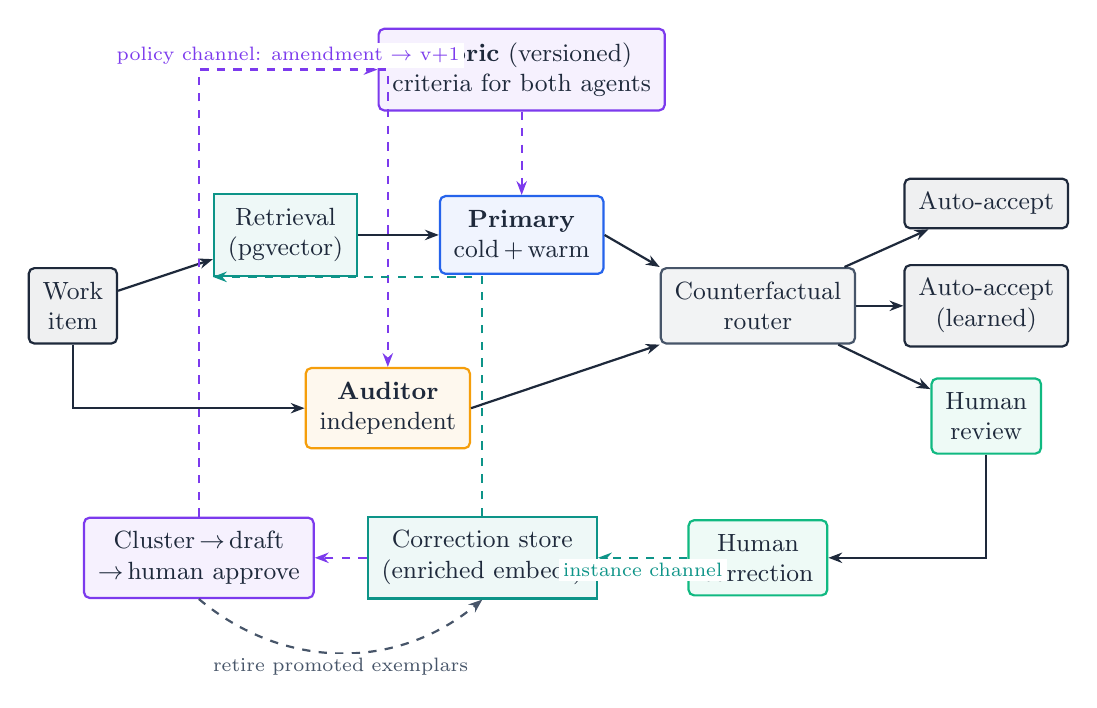
\begin{tikzpicture}[node distance=0pt]

  % --- Main pipeline ------------------------------------------------------
  \node[mzbox=mzInk]      (work)    at (0,0)        {Work\\item};
  \node[mzstore=mzVector] (retr)    at (2.7,0.9)    {Retrieval\\(pgvector)};
  \node[mzbox=mzPrimary]  (primary) at (5.7,0.9)    {\textbf{Primary}\\cold\,+\,warm};
  \node[mzbox=mzAuditor]  (auditor) at (4.0,-1.3)   {\textbf{Auditor}\\independent};
  \node[mzbox=mzRouter]   (router)  at (8.7,0)       {Counterfactual\\router};

  % rubric feeds both agents
  \node[mzbox=mzRubric]   (rubric)  at (5.7,3.0)     {\textbf{Rubric} (versioned)\\criteria for both agents};

  % outcomes
  \node[mzbox=mzInk]      (auto)    at (11.6,1.3)    {Auto-accept};
  \node[mzbox=mzInk]      (learned) at (11.6,0.0)    {Auto-accept\\(learned)};
  \node[mzbox=mzHuman]    (human)   at (11.6,-1.4)   {Human\\review};

  % --- Learning-loop band (bottom) ---------------------------------------
  \node[mzbox=mzHuman]    (fb)      at (8.7,-3.2)    {Human\\correction};
  \node[mzstore=mzVector] (cstore)  at (5.2,-3.2)    {Correction store\\(enriched embed.)};
  \node[mzbox=mzRubric]   (cluster) at (1.6,-3.2)    {Cluster\,$\to$\,draft\\$\to$\,human approve};

  % --- Pipeline edges -----------------------------------------------------
  \draw[mzedge] (work) -- (retr);
  \draw[mzedge] (retr) -- (primary);
  \draw[mzedge] (work.south) |- (auditor.west);   % auditor gets the item, NOT exemplars
  \draw[mzedge] (primary.east) -- (router.north west);
  \draw[mzedge] (auditor.east) -- (router.south west);
  \draw[mzedge] (router) -- (auto);
  \draw[mzedge] (router) -- (learned);
  \draw[mzedge] (router) -- (human);

  % rubric to both agents (policy reaches everyone)
  \draw[mzloop=mzRubric] (rubric.south) -- (primary.north);
  \draw[mzloop=mzRubric] (rubric.west) -| (auditor.north);

  % --- Instance channel (teal, dashed): correction -> store -> retrieval --
  \draw[mzedge] (human.south) |- (fb.east);
  \draw[mzloop=mzVector] (fb) -- (cstore)
        node[midway, below, font=\scriptsize, text=mzVector,
             fill=white, inner sep=1.5pt]{instance channel};
  \draw[mzloop=mzVector] (cstore.north) |- (retr.south west);

  % --- Policy channel (purple, dashed): cluster -> approve -> rubric ------
  \draw[mzloop=mzRubric] (cstore) -- (cluster);
  \draw[mzloop=mzRubric] (cluster.north) |- (rubric.west)
        node[pos=0.75, above, font=\scriptsize, text=mzRubric,
             fill=white, inner sep=1.5pt]{policy channel: amendment $\to$ v+1};
  \draw[mzloop=mzRouter] (cluster.south) to[out=-40,in=-140]
        node[midway, below, font=\scriptsize, text=mzRouter,
             fill=white, inner sep=1.5pt]{retire promoted exemplars} (cstore.south);

\end{tikzpicture}

\end{document}
